\documentclass[a4paper, 11pt]{article}
\usepackage[utf8]{inputenc} 
\usepackage[T1]{fontenc}
\usepackage{lmodern}
\usepackage{graphicx}

\usepackage[french]{babel}

\usepackage{xcolor}
\usepackage{listings}




% Source Code
%\usepackage{color}
%\usepackage{textcomp}
%\usepackage{listings}
%\usepackage{ulem}
%\usepackage[T1]{fontenc}
%\usepackage{times}
% \usepackage{needspace}
 

% Source Code
\usepackage{color}
\usepackage{textcomp}
\usepackage{listings}

\definecolor{source}{gray}{0.85}% my comment style
\newcommand{\myCommentStyle}[1]{{\footnotesize\sffamily\color{gray!100!white} #1}}
%\newcommand{\myCommentStyle}[1]{{\footnotesize\sffamily\color{black!100!white} #1}}

% my string style
\newcommand{\myStringStyle}[1]{{\footnotesize\sffamily\color{violet!100!black} #1}}
%\newcommand{\myStringStyle}[1]{{\footnotesize\sffamily\color{black!100!black} #1}}

% my symbol style
\newcommand{\mySymbolStyle}[1]{{\footnotesize\sffamily\color{violet!100!black} #1}}
%\newcommand{\mySymbolStyle}[1]{{\footnotesize\sffamily\color{black!100!black} #1}}

% my keyword style
\newcommand{\myKeywordStyle}[1]{{\footnotesize\sffamily\color{green!70!black} #1}}
%\newcommand{\myKeywordStyle}[1]{{\footnotesize\sffamily\color{black!70!black} #1}}

% my global style
\newcommand{\myGlobalStyle}[1]{{\footnotesize\sffamily\color{blue!100!black} #1}}
%\newcommand{\myGlobalStyle}[1]{{\footnotesize\sffamily\color{black!100!black} #1}}

% my number style
\newcommand{\myNumberStyle}[1]{{\footnotesize\sffamily\color{brown!100!black} #1}}
%\newcommand{\myNumberStyle}[1]{{\footnotesize\sffamily\color{black!100!black} #1}}

\lstset{
language={},
% characters
tabsize=3,
escapechar={!},
keepspaces=true,
breaklines=true,
alsoletter={\#},
literate={\$}{{{\$}}}1,
breakautoindent=true,
columns=fullflexible,
showstringspaces=false,
% background
frame=single,
aboveskip=1em, % automatic space before
framerule=0pt,
basicstyle=\footnotesize\sffamily\color{black},
keywordstyle=\myKeywordStyle,% keyword style
commentstyle=\myCommentStyle,% comment style
frame=single,%
backgroundcolor=\color{source},
% numbering
stepnumber=1,
numbersep=10pt,
numberstyle=\tiny,
numberfirstline=true,
% caption
captionpos=b,
% formatting (html)
moredelim=[is][\bfseries]{<b>}{</b>},
moredelim=[is][\textit]{<i>}{</i>},
moredelim=[is][\underbar]{<u>}{</u>},
moredelim=[is][\color{red}\uwave]{<wave>}{</wave>},
moredelim=[is][\color{red}\sout]{<del>}{</del>},
moredelim=[is][\color{blue}\underbar]{<ins>}{</ins>},
% smalltalk stuff
morecomment=[s][\myCommentStyle]{"}{"},
%    morecomment=[s][\myvs]{|}{|},
morestring=[b][\myStringStyle]',
moredelim=[is][]{<sel>}{</sel>},
moredelim=[is][]{<rcv>}{</rcv>},
moredelim=[is][\itshape]{<symb>}{</symb>},
moredelim=[is][\scshape]{<class>}{</class>},
morekeywords={true,false,nil,self,super,thisContext},
identifierstyle=\idstyle,
}

\makeatletter
\newcommand*\idstyle[1]{%
\expandafter\id@style\the\lst@token{#1}\relax%
}
\def\id@style#1#2\relax{%
\ifnum\pdfstrcmp{#1}{\#}=0%
% this is a symbol
\mySymbolStyle{\the\lst@token}%
\else%
\edef\tempa{\uccode`#1}%
\edef\tempb{`#1}%
\ifnum\tempa=\tempb%
% this is a global
\myGlobalStyle{\the\lst@token}%
\else%
\the\lst@token%
\fi%
\fi%
}
\makeatother


%\newcommand{\ct}{\lstinline[backgroundcolor=\color{white}]}
%\newcommand{\needlines}[1]{\Needspace{#1\baselineskip}}
\newcommand{\lct}{\texttt}

\lstnewenvironment{code}{%
    \lstset{%
    % frame=lines,
    frame=single,
    framerule=0pt,
    mathescape=false
    }%
    \noindent%
    \minipage{\linewidth}%
}{%
    \endminipage%
}%


\lstnewenvironment{codeWithLineNumbers}{%
    \lstset{%
    % frame=lines,
    frame=single,
    framerule=0pt,
    mathescape=false,
    numbers=left
    }%
    \noindent%
    \minipage{\linewidth}%
}{%
    \endminipage%
}%



\newenvironment{codeNonSmalltalk}
{\begin{alltt}\sffamily}
{\end{alltt}\normalsize}


 
\begin{document}

\section{Introduction}

Le projet Ironmines a été créé pour répondre offrir une interface de
programmation pour faire évoluer le robot Kobuki. L'objectif est
bien-sur de le faire concourir à la coupe de France de Robotique.

\section{Installation}

À partir d'une distribution Raspbian vierge il faudra installer les
dépendances suivantes :
\begin{itemize}
\item ROS - Kobuki
\item Rosserial (pour communiquer avec l'Arduino)
\item PhaROS - Ironmines
\end{itemize}

\subsection{ROS - Kobuki}

Tout d'abord il faut installer ROS sur le Raspberry : 

\begin{lstlisting}
  sudo sh -c 'echo "deb http://64.91.227.57/repos/rospbian wheezy main" > /etc/apt/sources.list.d/rospbian.list'
  wget http://64.91.227.57/repos/rospbian.key -O - | sudo apt-key add -

  sudo apt-get update

  sudo apt-get install ros-groovy-ros-comm
  sudo rosdep init
  rosdep update

  echo "source /opt/ros/groovy/setup.bash" >> ~/.bashrc
  echo "export ROS_HOSTNAME=localhost" >> ~/.bashrc
  source ~/.bashrc
\end{lstlisting}

Puis installer les noeuds pour communiquer avec le Kobuki : 

\begin{lstlisting}
  sudo apt-get install ros-groovy-kobuki-node 
  sudo apt-get install ros-groovy-kobuki-msgs
  sudo apt-get install ros-groovy-kobuki-ftdi
\end{lstlisting}

On pourra alors tester l'installation en exécutant dans un terminal :

\begin{verbatim}
  roscore
\end{verbatim}

Et dans un autre terminal : 

\begin{verbatim}
  roslaunch kobuki_node minimal.launch
\end{verbatim}

Si tout ce lance correctement, on peut passer à la suite.

\subsection{Rosserial}
  
\section{Architecture}

D'un façon générale, Pharo fait office d'intelligence. ROS ne fait que
transmettre les message provenant de l'Arduino et du Kobuki au travers
des noeuds Rosserial et Kobuki\_node.
\begin{center}
  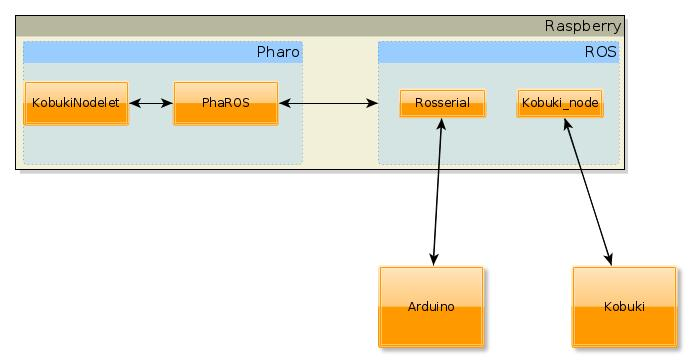
\includegraphics[width=\linewidth]{./architecture.jpg}
  \caption{Architecture générale}
  \label{archi_generale}
\end{center}
\subsection{Arduino}
Le code pour l'arduino se trouve a l'Url
:\\ https://github.com/mattonem/ironmines-arduino.git.

Basiquement, on utilise la librairie fournie par Rosserial pour
pouvoir publier différents topics sur le port serie ainsi que souscrire
a d'autre. On publie les données relatives au contacteur de démarrage
et au capteurs ultrasons. On souscrit aux différents topics concernant
les actions a effectuer (activer le canon, bouger le bras
retractable).

\subsubsection{Subscribed Topics}

\begin{itemize}
\item  todo
\end{itemize}

\subsubsection{Published Topics}

\begin{itemize}
\item \texttt{/sonar/<i> (std\_msgs/UInt16)}\\
  Donne la distance au mur en face du sonar i.
\item \texttt{/startTrigger (std\_msgs/Bool)}\\ 
  Donne les fronts montant et descendant pour le cordon de demarrage.
\end{itemize}

\end{document}
